\documentclass{article}
\usepackage{amssymb}
\usepackage{amsmath}
\usepackage[utf8]{inputenc}
\usepackage[margin=1in]{geometry}
\usepackage{graphicx}

\newcommand{\vap}[1]{\text{VAP}^\text{#1}}
\newcommand{\cvap}[1]{\text{CVAP}^\text{#1}}

\title{CVAP Estimation}
\author{Christopher Wolfram, Moon Duchin, Aaron Schein}
\date{August 2024}

\begin{document}

\maketitle

\section{The Problem}
Our goal is to generate block-level CVAP estimates for race/ethnicity categories that are relevant for litigation. This poses two challenges:
\begin{enumerate}
    \item Citizenship data is only available from the ACS at the block group or tract level, and not for blocks.
    \item The race/ethnicity categories used by the ACS for citizenship data are different from those that are relevant for litigation.
\end{enumerate}

\section{Disaggregating From Tracts to Blocks With Small Area Estimation}
Our basic approach is to estimate the citizenship rate on tracts with ACS data, and then apply that citizenship rate to block-level VAP data from the decennial Census.

We compute the disaggregated estimates for each race/ethnicity category independently, so this section will not make reference to race/ethnicity categories. Everything described will be be recomputed for each category.

We use tracts instead of block groups because, though the ACS provides CVAP on block groups, it doesn't appear to provide VAP, which makes it difficult to compute citizenship rates on geographies smaller than tracts.

\subsection{Terms}

\begin{align*}
    b &: \text{Census block} \\
    t &: \text{Census tract} \\
    % TODO: Is there better notation for t_b? It is a bit confusing to have t and t_b.
    t_b &: \text{Census tract containing $b$} \\
    \vap{dec}_b &: \text{Decennial Census estimate of VAP in $b$} \\
    \vap{ACS}_t &: \text{Decennial Census estimate of VAP in $t$} \\
    \cvap{ACS}_t &: \text{Decennial Census estimate of CVAP in $t$}
\end{align*}

\subsection{Discounted VAP}
A simplified version of our model would be $$\cvap{}_b = \vap{dec}_b \frac{\cvap{ACS}_{t_b}}{\vap{ACS}_{t_b}}$$ where the CVAP of the block $b$ is estimated by multiplying the citizenship rate (among voting-age people) of the surrounding tract $t_b$ by the voting-age population of the block $b$.

However, this Discounted VAP approach has issues when $\vap{ACS}_{t_b}$ is small, as the estimate of the citizenship rate will have high variance. Even worse, when $\vap{ACS}_{t_b} = 0$ there is no meaningful estimate of the citizenship rate.

\subsection{Bayesian CVAP}

We use Bayesian methods to model uncertainty while using the same basic approach as in Discounted VAP. Our model is:
\begin{align*}
    C_t &\sim \text{Beta}(\alpha, \beta) \\
    \cvap{ACS}_t &\sim \text{Binomial}(\vap{ACS}_t, C_t) \\
    \cvap{}_b &\sim \text{Binomial}(\vap{dec}_b, C_{t_b})
\end{align*}
$C_t$ represents the citizenship rate in the tract $t$. We use a beta distribution prior for $C_t$ with parameters $\alpha$ and $\beta$ that are estimated with MLE for each state. By beta-binomial conjugacy, the posterior estimates for $C_t$ and $\cvap{}_b$ are
\begin{align*}
    C_t \mid - &\sim \text{Beta}(\alpha + \cvap{ACS}_t, \beta + \vap{ACS}_t - \cvap{ACS}_t) \\
    \cvap{}_b \mid - &\sim \text{BetaBinonial}(\vap{dec}_b, \alpha + \cvap{ACS}_{t_b}, \beta + \vap{ACS}_{t_b} - \cvap{ACS}_{t_b})
\end{align*}
Looking at the form of $C_t$ shows the relation ot Discounted VAP. When $\vap{ACS}_t$ or $\cvap{ACS}_t$ are large, the $\alpha$ and $\beta$ terms will be drowned out, and $C_t$ will tend toward a spike at $\cvap{ACS}_t / \vap{ACS}_t$. However, when $\vap{ACS}_t$ and $\cvap{ACS}_t$ are small, $C_t$ will tend toward $\text{Beta}(\alpha, \beta)$ which essentially represents the statewide distribution of tract citizenship rates.

\section{Estimating for Litigation Race/Ethnicity Categories}
Before fitting the model above, we first generate tract-level estimates of VAP and CVAP for the litigation race/ethnicity categories. These litigation VAP and CVAP estimates are then used as inputs into the Bayesian CVAP model.

Our basic approach to to compute linear combinations of the ACS categories with weights that come from the Decennial Census.

\subsection{Litigation Categories}
\begin{itemize}
    \item Black or African-American Alone or in Combination
    \item Hispanic or Latino (but not in the above category)
    \item Asian or Native Hawaiian or Pacific Islander Alone or in Combination (but not in the above categories)
    \item American Indian or Alaska Native Alone or in Combination (but not in the above categories)
    \item Some Other Race Alone or in Combination (but not in the above categories)
    \item White Alone, Not Hispanic or Latino
\end{itemize}

\subsection{Litigation Category Estimation}
Let $\text{B}$ represent the ACS Black or African-American Alone, $\text{B}+$ represent the litigation Black or African-American Alone or in Combination category, $\text{2+}$ the ACS Two Or More Races category, $\text{H}+$ the ACS Hispanic or Latino category, and so on. Also let $N_\text{VAP}(c)$ represent the ACS estimate for the voting age population of the category $c$, and $N_\text{CVAP}(c)$ the same for citizen voting age population. Also let $p(c_1 \mid c_2)$ represent the proportion of the voting age population in category $c_2$ who are also in $c_1$ as computed with data from the Decennial Census.

\subsubsection{Black or African-American Alone or in Combination}
We estimate the Black or African-American Alone or in Combination VAP and CVAP on tracts with $$N_\text{VAP}(\text{B+}) \approx \underbrace{N_\text{VAP}(\text{B})}_\text{ACS}+\underbrace{N(\text{2+})_\text{VAP}}_\text{ACS} \underbrace{p(\text{B+}\mid\text{2+})}_\text{Decennial}$$ and $$N_\text{CVAP}(\text{B+}) \approx \underbrace{N_\text{CVAP}(\text{B})}_\text{ACS}+\underbrace{N(\text{2+})_\text{CVAP}}_\text{ACS} \underbrace{p(\text{B+}\mid\text{2+})}_\text{Decennial}$$ The Decennial term could be naively be computed with $$p(\text{B+}\mid\text{2+}) = \frac{p(\text{B+}, \text{2+})}{p(\text{2+})}$$ However, if $p(\text{2+})$ is very small, then this estimate has high variance. This is the same as the problem with Discounted VAP above, and we solve it by using the same Bayesian beta-binomial model to estimate the proportion of voting age people in $\text{2+}$ who are also in $\text{B+}$. (See figure \ref{fig:venn1}.)

Because the VAP and CVAP formulae are essentually the same, in later sections I will simply write $N(c)$ which can be substituted with $N_\text{VAP}$ or $N_\text{CVAP}$ to get the estimate for VAP or CVAP.

\begin{figure}
    \centering
    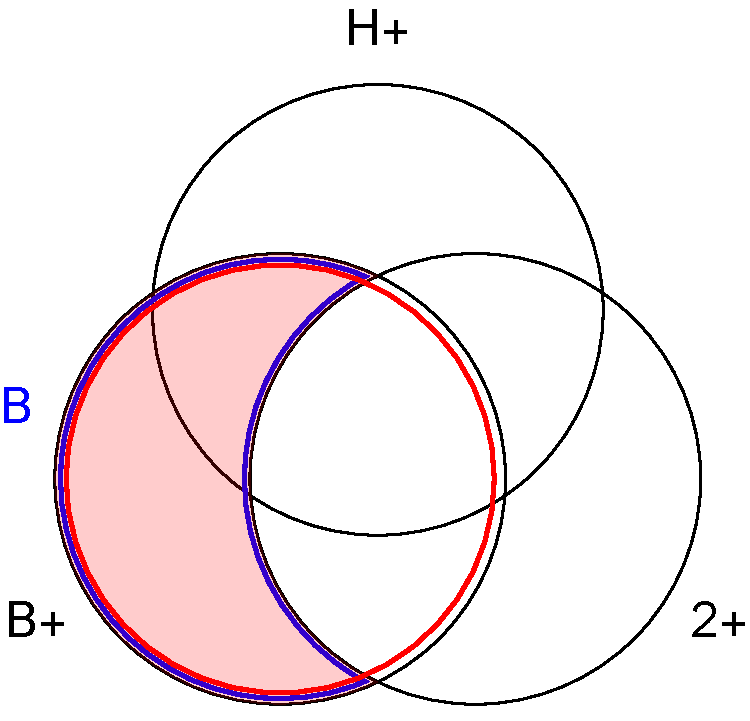
\includegraphics[width=0.5\linewidth]{vennDiagram1.pdf}
    \caption{Venn diagram for computing VAP and CVAP among Black or African-American Alone or in Combination. The red shaded region represents the ACS Black or African-American Alone category. The red outlined region represents the target Black or African-American Alone or in Combination category.}
    \label{fig:venn1}
\end{figure}

\subsubsection{Hispanic or Latino (but not in the above category)}
We similarly estimate the litigation Hispanic or Latino category with $$N(\text{H+})-N(\text{H+})p(\text{B+}\mid\text{H+})$$
(See figure \ref{fig:venn2}.)

\begin{figure}
    \centering
    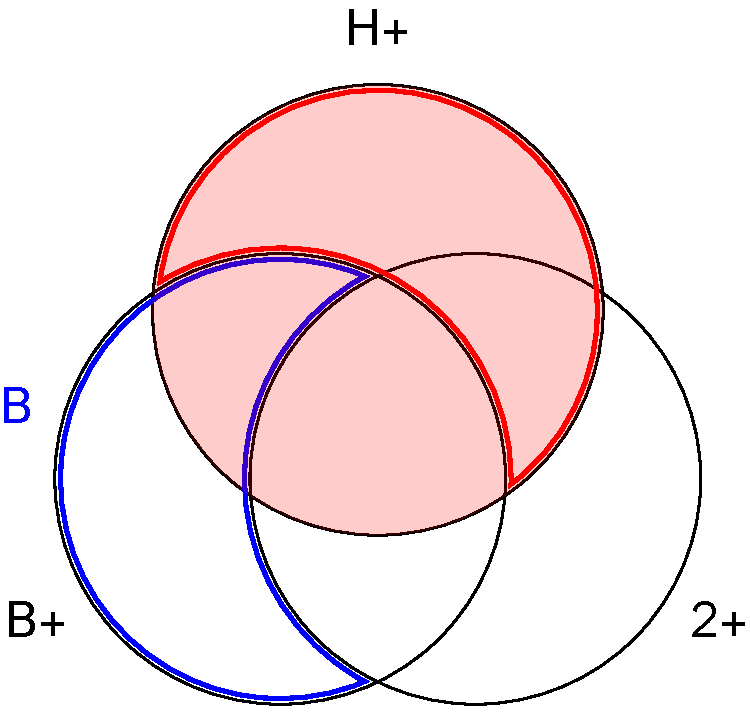
\includegraphics[width=0.5\linewidth]{vennDiagram2.pdf}
    \caption{Venn diagram for computing VAP and CVAP for the litigation Hispanic or Latino category. The red shaded region represents the ACS Hispanic or Latino category. The red outlined region represents the target litigation Hispanic or Latino category. The blue outlined region represents the ACS Black or African-American Alone category.}
    \label{fig:venn2}
\end{figure}

\subsubsection{$X$ Alone or in Combination (but not in the above categories)}
For all other categories, let $X$ represent an ACS category (such as Some Other Race Alone) and $X+$ represent the analogous litigation category (such as Some Other Race Alone or In Combination (but not in the above categories)).

We have two ways of estimating VAP and CVAP for these race/ethnicity categories:
$$N(X+) \approx N(\text{X}) - N(\text{X})p(\text{H+} \mid \text{X}) + N(\text{2+})p(\text{T} \mid \text{2+})$$
$$N(X+) \approx N(\text{X}) - N(\text{H+})p(\text{X} \mid \text{H+}) + N(\text{2+})p(\text{T} \mid \text{2+})$$
These two options amount to different assumptions about the citizenship rate among the voting age population of the overlap category that is in $X$ and Hispanic or Latino. The first formula assigns the overlap population the citizenship rate among $X$, while the second assigns the citizenship rate among the ACS Hispanic or Latino category. (See figure \ref{fig:venn3}.)

\begin{figure}
    \centering
    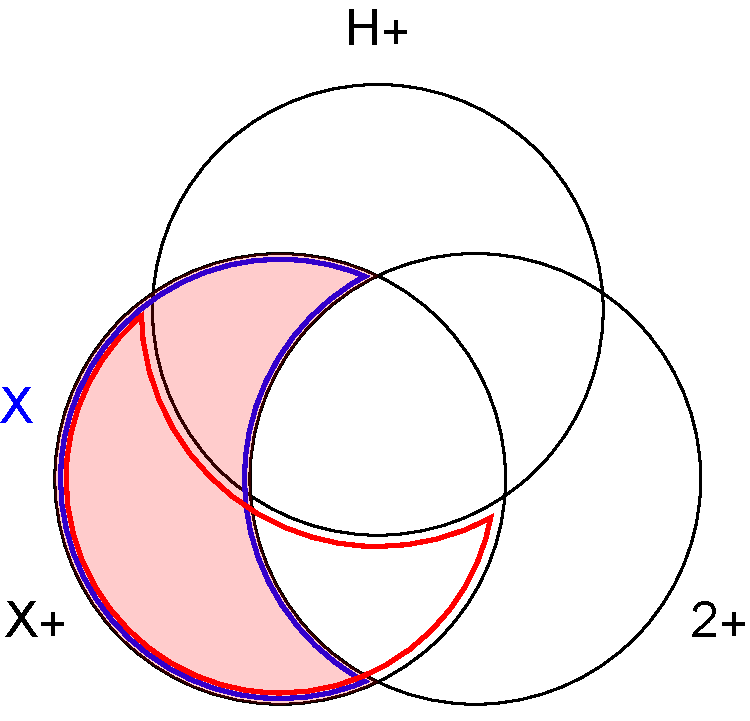
\includegraphics[width=0.5\linewidth]{vennDiagram3.pdf}
    \caption{Venn diagram for computing VAP and CVAP for the litigation $X+$ category. The red shaded region represents the ACS $X$ category. The red outlined region represents the target litigation $X+$ category.}
    \label{fig:venn3}
\end{figure}

\subsubsection{White Alone, Not Hispanic or Latino}
This is the only litigation category that is provided directly by the ACS.

\subsection{Validation}
The White Alone, Not Hispanic or Latino category is given to us by the ACS. However, if we use the same methods to estimate it that we used above to estimate non-Hispanic versions of other categories, we should get results that match the numbers we get directly from the ACS. Unfortunately, this is not what we see.

Critically, it appears that the ACS and Decennial Census have very different counts for the overlap category containing the White Alone and Hispanic or Latino population (that is, the intersection population). We can estimate the size of this population from the ACS by subtracting the White Alone population totals with the White Alone, Not Hispanic or Latino totals. Comparing those with the population given in the Decennial Census gives figure \ref{fig:decACSscatter}, which unfortunately does not show a good match.

\begin{figure}
    \centering
    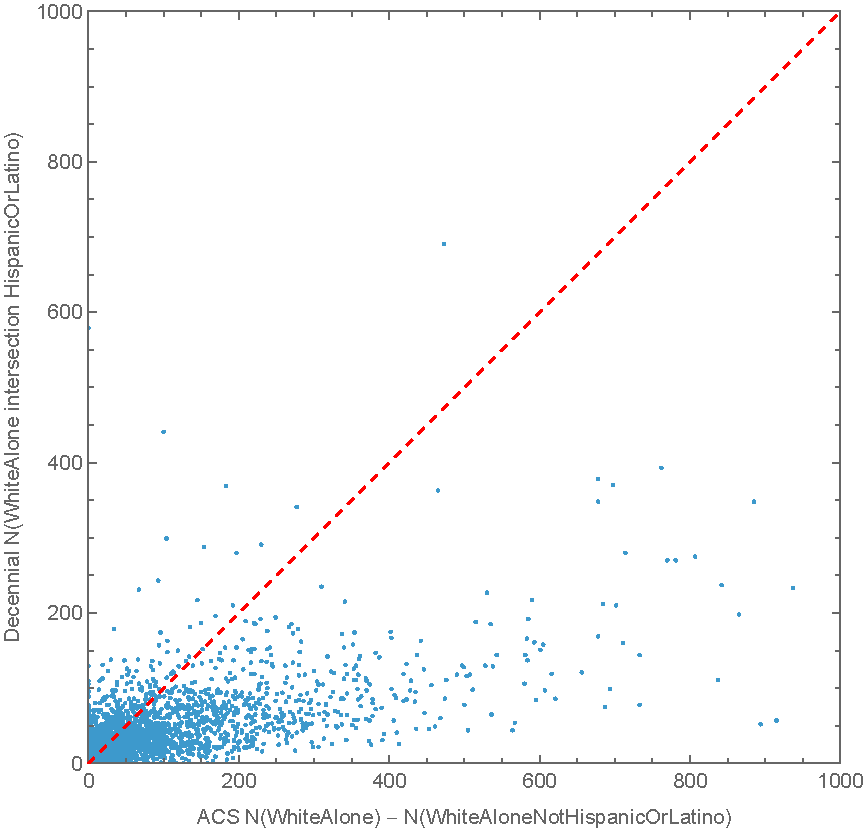
\includegraphics[width=0.7\linewidth]{decACSscatter.pdf}
    \caption{Scatter plot comparing ACS estimates of the White Alone $\cap$ Hispanic or Latino voting age population with the Decennial Census. Each point represents a tract in Georgia. The red dashed line indicates a slope of 1, which the scatter plot does not appear close to.}
    \label{fig:decACSscatter}
\end{figure}

This discrepancy can be further seen by comparing the histograms of the White Alone $\cap$ Hispanic or Latino VAP among tracts in Georgia, computed both from the ACS and Decennial Census (see figure \ref{fig:decACShist}). The ACS and Decennial Census histograms look very different. The left side of the histogram might be partially explainable through rounding, but the long tail that the ACS shows (and the Decennial Census does not) is harder to explain with rounding alone.

\begin{figure}
    \centering
    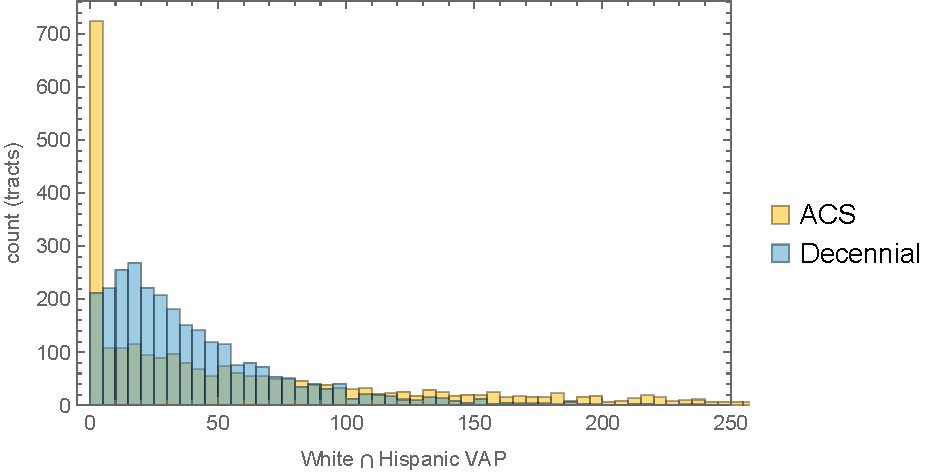
\includegraphics[width=0.7\linewidth]{decACShist.pdf}
    \caption{Histogram showing the distribution of the White Alone $\cap$ Hispanic or Latino VAP among tracts in Georgia, computed both from the ACS and Decennial Census. Note that the ACS has a differently shaped tail from the Decennial Census.}
    \label{fig:decACShist}
\end{figure}

\end{document}
